\documentclass[openany]{book}
\usepackage[T1]{fontenc}
\usepackage[utf8x]{inputenc}
\usepackage[english,hebrew]{babel} % Typographical (and other) rules
\usepackage[a4paper,left=24.8mm,top=27.4mm,headsep=2\baselineskip,textwidth=107mm,marginparsep=8.2mm,marginparwidth=49.4mm,textheight=49\baselineskip,headheight=\baselineskip,asymmetric]{geometry}
\usepackage{siunitx,mathtools}
\begin{document}
\selectlanguage{english}
$$\SI{1}{\electronvolt}=\SI{1.602e-19}{\joule}$$
In our experiments, the gas pressure inside the capillary was on the order of \numrange[range-phrase = --]{10}{20} bars, or \numrange[range-phrase = --]{7}{15} Torr.
\begin{description}
\item[Electrical  breakdown] of air occurs when the electric field reaches a strength of about \SI{3e6}{\volt\per\m}. In fields this strong, electrons are ripped from molecules in the air. They are then accelerated by thefield and collide with other molecules, knocking electrons out of these molecules,  and  so  on,  in  a  cascading  process.  The  result  is  a spark, because eventually the electrons will combine in a more friendly manner with molecules and drop down to a lower energy level, emitting the light that you see.
\item[Debye Length] Beyond a Debye shpere, the plasma remains effectively neutral. $\lambda_D$ is also a measure of the penetration depth of external electrostatic fields, i.e. of the thickness of the boundary sheath over which charge neutrality may not be maintained.

\item[Plasma Parameter] The plausibility of the argument used to establish the derivation to Debye length requires that a large number of electrons be present within the Debye sphere, i.e. $N_e \lambda_D^3\gg1$. Broadly speeking, the more particles there are in the Debye sphere the less likely it is that there will be a significant resultant force on any given particle due to "collisions". It is, therefore, a measure of the dominance of collective interactions over collisions. The most fundamental of there collective interactions are the plasma oscillations.
\item[plasma oscillations] A response to charge imbalance. The strong electrostatic fields which drive the electrons to re--establish neutrality cause oscillations about the equilibrium position at a characteristic frequency $\omega_p$. Since the imbalance occurs over a distance $\lambda_D$ and the electron thermal speed $v_e$ is typically $\sqrt{k_B T_e/m_e}$ we may express the electron plasma frequency $\omega_{pe}$ by
$$\omega_{pe}=\frac{\sqrt{k_B T_e / m_e}}{\lambda_D}=\sqrt{\frac{N_e e^2}{m_e \varepsilon_0}}$$
Notice that any applied fields with frequencies less than the electron plasma frequency are prevented from penetrating the plasma by the more rapid electron response which neutralizes the field. Thus a plasma is not transparent to electromagnetic radiation of frequency $\omega < \omega_p $. The corresponding frequency for ions, the ion plasma frequency $\omega_{pi}$, is defined by 
$$\omega_{pi}=\sqrt{\frac{n_i (Z e)^2}{m_i \varepsilon_0}}\simeq \sqrt{n_i/A}$$
where $Z$ denots the charge state and $A$ the atomic number.
\item[Collisions and the plasma parameter] We have seen that the effective range of an electric field, and hence of a collision, is the Debye length. Thus any particle interacts at any instant with the large number of particles in its Debye sphere. Plasma collisions are therefore \emph{many}--body interactions and since $\Lambda \gg 1$, collisions are predominantly weak. This is in sharp contrast with the strong, binary collisions that characterize a neutral gas.
\item[$T_e$ and $N_e$]
Under what conditions the term 'temperature' has any significant meaning. In the kinetic theory of gases the equilibrium velocity distribution of particles is Maxwellian, from which the kinetic temperature
is derived.  In order for the statistics of this process to be valid, the mean free path
for particle collisions must be far smaller than the dimensions of the containing
vessel and the time between collisions must be short compared with other characteristic times, such as those for particle heating and containment.
Usually in laboratory plasmas the electron--electron mean free path and collisional relaxation times are such that the free electrons do have a Maxwellian
velocity distribution to which an electron temperature $T$, can be ascribed.
This is often not the case for ions and then the ion kinetic temperature has no
meaning.
\item[sound speed in a plasma]
$$\frac{\omega}{k}=\sqrt{\frac{\gamma_e k_{B}T_{e}+\gamma_{i}k_{B}T_{i}}{M}}$$
\item[Doppler Broadening]
$$P\left(\varepsilon\right)=\frac{e^{-\beta\varepsilon}}{Z},\ \varepsilon=\frac{p^{2}}{2m}=\frac{1}{2}mv_{x}^{2}\Rightarrow P\left(v_{x}\right)=A\cdot\frac{e^{-\beta\frac{1}{2}mv_{x}^{2}}}{Z}$$

$$\frac{f}{f_{0}}=1+\frac{v_{x}}{c}\Rightarrow v_{x}=\frac{c}{f_{0}}\left(f-f_{0}\right)P\left(f\right)=A\cdot e^{-\beta\frac{1}{2}\frac{mc^{2}}{f_{0}^{2}}\left(f-f_{0}\right)^{2}}$$

$$1=\int_{0}^{f_{max}}P\left(f\right)\mathrm{d}f$$
Since $mc^{2}\gg k_{B}T$, $f_{max}\approx\infty$ and the lower limit may be approximated to $-\infty$.
$$1=\int_{-\infty}^{\infty}P\left(f\right)\mathrm{d}f=A\int_{-\infty}^{\infty}e^{-\beta\frac{1}{2}\frac{mc^{2}}{f_{0}^{2}}\left(f-f_{0}\right)^{2}}\mathrm{d}f\Rightarrow A=\sqrt{\frac{mc^{2}}{2\pi k_{B}T}}\frac{1}{f_{0}}$$
\item[speed of sound]
In a neutral gas:
\begin{align*}
  \frac{\omega}{k} &= \sqrt{\frac{\gamma p_{0}}{\rho_{0}}}=\sqrt{\frac{\gamma k_{B}T}{M}}\equiv c_{s} & \gamma &= (2+N)/N
\end{align*}
$\gamma$ is the adiabatic constant. $N$ is the number of degrees of freedom.

At room temperature, where thermal energy is fully partitioned into rotation (rotations are fully excited) but quantum effects prevent excitation of vibrational modes, the value is 7/5 = 1.4 for diatomic molecules, according to kinetic theory.

Ion acoustic waves:
$$\frac{\omega}{k}=\sqrt{\frac{\gamma_e k_B T_e+\gamma_i k_B T_i}{M}}\approx \sqrt{\frac{\gamma_e k_B T_e}{M}} \equiv v_{s}$$
The electrons move so fast relative to these waves that they have time to equalize their temperature everywhere; therefore, the electrons are isothermal, and $\gamma_e=1$.

Since the ions suffer one-dimensional compressions in the plane waves we have assumed, $\gamma_i=3$.

In laboratory plasmas, in which the condition $T_i\ll T_e$ is common, the sound speed $v_s$ depends on electron temperature and on ion mass. For $T_e\sim \SI{1}{\electronvolt}$, $v_s \sim \SI{e6}{\cm\per\sec}$.
\end{description}
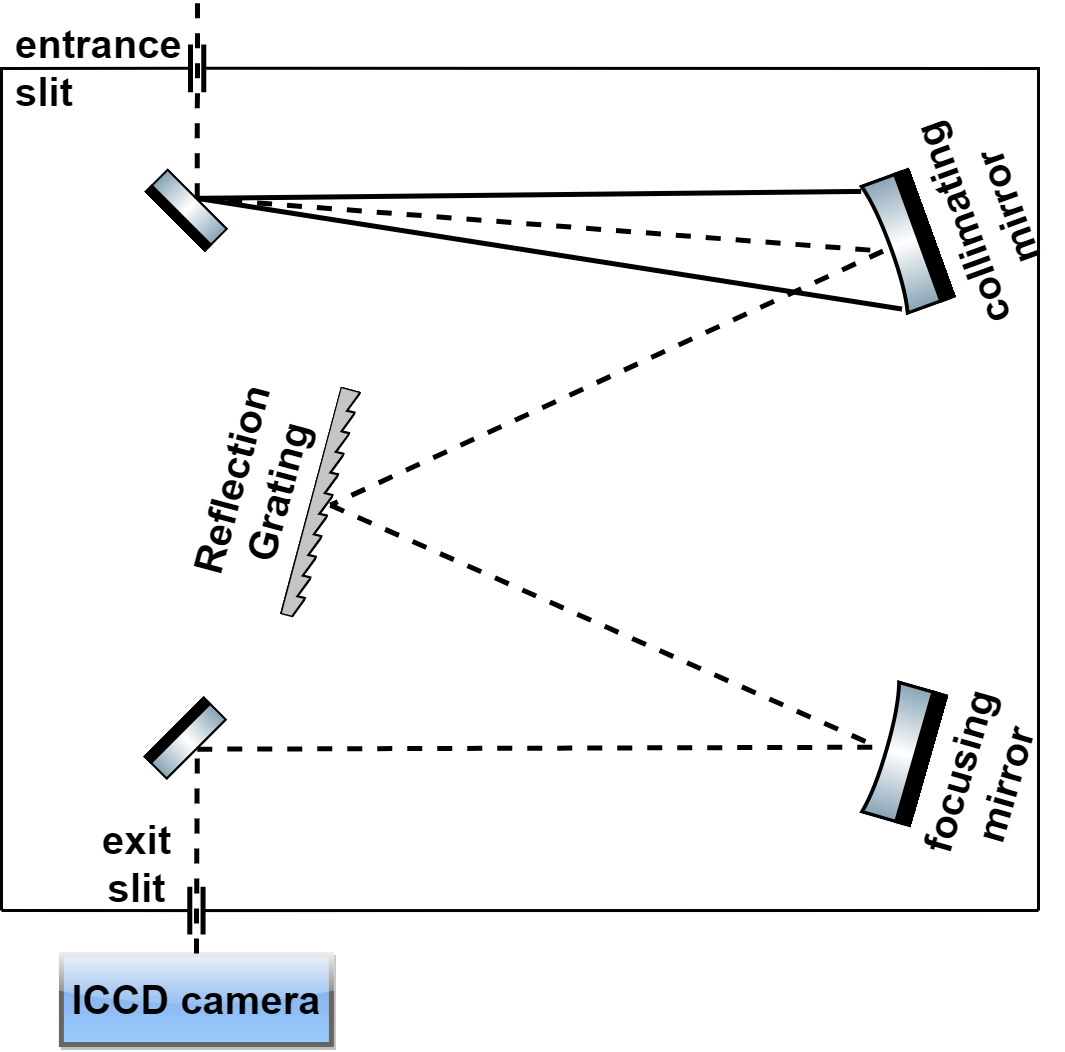
\includegraphics[width=\textwidth]{figures/results/spectro/spectrometer.png}
\end{document}
